\documentclass[12pt]{article}
\usepackage{amsmath}
\usepackage{amssymb}
\usepackage{fancyhdr}
\usepackage{graphicx}
\usepackage{pdfpages}
\usepackage{listings}
\usepackage{color}
\usepackage{lmodern}
\usepackage{hyperref}

\definecolor{dkgreen}{rgb}{0,0.6,0}
\definecolor{gray}{rgb}{0.5,0.5,0.5}
\definecolor{mauve}{rgb}{0.58,0,0.82}
\pagestyle{headings}
\setlength{\oddsidemargin}{0in}
\setlength{\evensidemargin}{0in}
\setlength{\textheight}{9in}
\setlength{\textwidth}{6.5in}
\setlength{\topmargin}{-0.5in}
\setlength{\headheight}{14pt}
\renewcommand*\rmdefault{lmss}
\renewcommand*\contentsname{Table of Contents}
\lstset{language=Matlab,
	aboveskip=3mm,
	belowskip=3mm,
	showstringspaces=false,
	basicstyle={\normalfont\ttfamily},
	numbers=left,
	numberstyle=\tiny\color{gray},
	keywordstyle=\color{blue},
	commentstyle=\color{dkgreen},
	stringstyle=\color{mauve},
	breaklines=true,
	breakatwhitespace=true,
	tabsize=4
}

\newcommand{\horizontalLine}{
	\begin{center}
		\hrule width 1.0\textwidth
	\end{center}
}

\newcommand{\smallHorizontalLine}{
    \begin{center}
        \hrule width 0.5\textwidth
    \end{center}}

%%%%%%%%%%%%%%%%%%%%%%%%%%%%%%%%%%%%%%%%%%%%%%%%%%%%%%%%%%
%%%%%%%%%%%%%%%%%%%%%%%%%%%%%%%%%%%%%%%%%%%%%%%%%%%%%%%%%%
\title{\vspace{-3ex}\bf Final Project Report\\[2ex] 
       \normalsize ECS 171: Machine Learning\\Fall 2015}
\date{\today}
\author{\bf Team Name: The Muses\\ \bf William Otwell (997371020)\\ \bf Marshall Hampson ()\\ \bf Nicholas Layton (996933702)\\ \bf Steven Mackey ()\\ \bf Amos Too ()\\ \bf Michael Fiueroa ()\\ \bf Peggy Li ()}

%%%%%%%%%%%%%%%%%%%%%%%%%%%%%%%%%%%%%%%%%%%%%%%%%%%%%%%%%%
%%%%%%%%%%%%%%%%%%%%%%%%%%%%%%%%%%%%%%%%%%%%%%%%%%%%%%%%%%
\begin{document}
\maketitle
\pagebreak
\tableofcontents
\pagebreak

%%%%%%%%%%%%%%%%%%%%%%%%%%%%%%%%%%%%%%%%%%%%%%%%%%%%%%%%%%
%%%%%%%%%%%%%%%%%%%%%%%%%%%%%%%%%%%%%%%%%%%%%%%%%%%%%%%%%%
\section{Abstract}
\label{sec:abstract}
Music lovers worldwide are in constant search of new sounds to enrich their music library. Many analytic applications have risen to popularity as a result of listeners' need for music discovery. Most of these applications utilize machine learning techniques to make recommendations and predictions for their users. One of the more common problems in music analytics is the process of recommending an enjoyable song or artist to a user based on their previous music choices. Another popular problem is the generation of a personalized playlist for a user, again based on their listening choices. 

We sought to perform predictive analytics on songs based on their acoustic qualities. We hoped to discover any relationship between a song's acoustic qualities and its inaudible qualities, such as genre or popularity. Ultimately, we constructed models to perform different types of analysis, depending on the complexity and structure of the problems. 

%%%%%%%%%%%%%%%%%%%%%%%%%%%%%%%%%%%%%%%%%%%%%%%%%%%%%%%%%%
%%%%%%%%%%%%%%%%%%%%%%%%%%%%%%%%%%%%%%%%%%%%%%%%%%%%%%%%%%
\horizontalLine
\section{Introduction}
\label{sec:introduction}

\subsection{Background}
\label{subsec:background}
The motivation to develop "smarter" software for music analytics originates largely from a desire to sell more products to customers. Some of the biggest players in the industry, Amazon and Apple, are notoriously known for their "genius" recommendations on what customers ought to buy next. Brian Whitman, co-founder and CTO of the Echo Nest, said in his article titled \textit{How music recommendation works - and doesn't work} that, "Amazon is not optimizing for the noble work of raising independent artists' profiles to the public, and they're definitely not optimizing for a good musical experience. They're statistically optimizing to make more money, to sell you more things." Brian also discusses how many radio companies, like Pandora, utilize popularity to provide an enjoyable radio-listening experience. Brian goes on to elaborate on the importance of not only focusing on the money-making techniques, but satisfying the need of listeners by focusing on the actual music, its sound waves and lyrical significance. 

Our approach to music analytics was similar to that of Brian Whitman's company, minus the lyrical analysis. We utilized data that represented the actual sound of the music, an approach that Brian calls "acoustic analysis." Some of the features that we included in our analysis, for example, were time signature, loudness, and key, to name a few. While most music analysis applications are geared towards popularity and sales, we hoped to focus our analysis on the sounds of the music and how the features of a song itself could provide predictive information.
\\
\\
The specific goals we hoped to accomplish were:
\begin{itemize}
    \item Predict the popularity of a song:
    \vspace{-3.5mm}
    \begin{itemize}
        \item Apply linear regression techniques to quantify and predict the popularity of a song based on its acoustic features
        \vspace{-3.5mm}
    \end{itemize}
    \item Classify a song into its genre(s)
    \vspace{-3.5mm}
    \begin{itemize}
        \item Utilize artificial neural networks to learn about the potential relationship between a song's acoustic qualities and its associated genres 
        \vspace{-3.5mm}
    \end{itemize}
    \item Discover trends in the songs regarding hotness and genre
    \vspace{-3.5mm}
    \begin{itemize}
        \item Utilize clustering techniques to discover trends in a songs features that might indicate a songs "hotness"
    \end{itemize}
\end{itemize}

The specific details for achieving each of the above goals are provided in Section~\ref{sec:methods}. 

\subsection{Million Song Dataset}
\label{subsec:datasetIntro}
The dataset that we chose to use is known as the Million Song Dataset. Rather than actually using a million songs, we used a small, manageable subset of the Million Song Dataset. For both the Neural Networks approach (Section~\ref{subsec:ann}) and the Clustering approach (Section~\ref{subsec:clustering}), we used the following features:
\begin{enumerate}
    \item danceability
    \vspace{-3.5mm}
    \item duration
    \vspace{-3.5mm}
    \item end of fade in
    \vspace{-3.5mm}
    \item energy
    \vspace{-3.5mm}
    \item key
    \vspace{-3.5mm}
    \item loudness
    \vspace{-3.5mm}
    \item mode
    \vspace{-3.5mm}
    \item song hotness
    \vspace{-3.5mm}
    \item start of fade out
    \vspace{-3.5mm} 
    \item tempo
    \vspace{-3.5mm}
    \item time signature
    \vspace{-3.5mm}
    \item year
\end{enumerate}

In addition to the list above, the Neural Networks approach also utilized a feature called "artist terms," which is simply a list of tags (also known as genres in our case) for each song. 
\\
\\
NOTE: LINEAR REGRESSION SHOULD INCLUDE ANY CHANGES THEY HAVE TO THIS LIST OF FEATURES. AS FAR AS I KNOW, THEY ARE USING THE SAME FEATURES

%%%%%%%%%%%%%%%%%%%%%%%%%%%%%%%%%%%%%%%%%%%%%%%%%%%%%%%%%%
%%%%%%%%%%%%%%%%%%%%%%%%%%%%%%%%%%%%%%%%%%%%%%%%%%%%%%%%%%
\horizontalLine
\section{Methods}
\label{sec:methods}

%%%%%%%%%%%%%%%%%%%%%%%%%%%%%%%%%%%%%%%%%%%%%%%%%%%%%%%%%%
\subsection{Linear Regression: Song Popularity}
\label{subsec:linearRegression}
In an effort to study the predictability of song "hotness" (a measure of popularity included in our data), we used linear regression and various feature sets to create a model. We began with feature reduction, using Lasso regression and Pricipal Component Analyses followed by normal linear regression. As in other sections, we started with the same features, but with danceability and energy removed. We also selectively used elements with a listed hotness of 0. Such an absolute value suggests missing data more than complete dearth of popularity, so we removed it in some regressions. We also tested the use of different number of song tags. Using a list sorted by number of appearances in the data, we examined the effects of using the full list, only the top 20 elements, and only the top 5. We represented these song tags as a matrix in which the rows are associated with sample and the columns with the different song tags. Every $m \times n$ element in the matrix contains a binary value representing the presence or absence of the corresponding song tag in the data pertaining to that row element.

We found that the overwhelming important factors in creating an accurate model were the presence and number of song tags, and avoiding overfitting with more complicated feature reduction techniques. The highest mean squared error we found was when we used Lasso regression, followed by our PCA driven attempt. In the end our best result came from retaining a modest number of song tags (20), using normal linear regression, and removing elements with a listed hotness of 0.

%%%%%%%%%%%%%%%%%%%%%%%%%%%%%%%%%%%%%%%%%%%%%%%%%%%%%%%%%%%%%
\subsection{Artificial Neural Networks: Song Genres}
\label{subsec:ann}
We utilized Neural Networks to predict song genres based on features of a song. Many songs, however, belonged to several genres. To represent the various genres, also known as tags, for a particular song, we formed a feature column for each possible tag in our dataset. Then, we scanned through each song to determine its set of tags and set the index of each tag to a 1 in the appropriate column if the tag was present for the particular song. If there were $n$ possible tags in the entire dataset, and $m$ samples, then the matrix needed to represent all tags for all samples would be an $m \times n$ matrix. Ultimately, our data matrix looked something like this:
\begin{equation}
    X = \begin{Bmatrix}
    	x^{(1)}_1 & x^{(1)}_2 & ... & x^{(1)}_{n_1} \\
    	x^{(2)}_1 & x^{(2)}_2 & ... & x^{(2)}_{n_1} \\
    	...       & ...       & ... & ... \\
        x^{(m)}_1 & x^{(m)}_2 & ... & x^{(m)}_{n_1} \\
    \end{Bmatrix},
    \\
    Y = \begin{Bmatrix}
    y^{(1)}_1 & y^{(1)}_2 & ... & y^{(1)}_{n_2} \\
    y^{(2)}_1 & y^{(2)}_2 & ... & y^{(2)}_{n_2} \\
    ...       & ...       & ... & ... \\
    y^{(m)}_1 & y^{(m)}_2 & ... & y^{(m)}_{n_2} \\
    \end{Bmatrix},
    \\
    D = \{X,Y\}
\end{equation} 
\begin{equation}
    x^{(i)}_j \in \Re
\end{equation}
\begin{equation}
    y^{(i)}_j \in \{0, 1\}
\end{equation}

where $n_1$ is the number of features, $n_2$ is the number possible tags, and $m$ is the number of samples.

We quickly found that if we included all of the possible tags from our dataset that the number of tags would reach an unmanageable amount. Training our network with such a large number of tags was computationally intensive and was difficult for our network to learn such a complex distribution. Instead, we decided to limit the number of tags to a small subset of the most popular tags. We were able to import a list of the 300 most popular genres in the dataset and use it as the limiting set of possible tags for our dataset. We found that even 300 tags was too many. Later, we found that limiting the possible number of tags would reduce error and misclassification rate.

By having 12 song features and $n_2$ possible genres, we knew we would need to construct a neural network with 12 input nodes and $n_2$ output nodes. The more complicated issue arose when we tried determining the adequate number of hidden nodes.

We were mostly interested in observing the effect of 3 different parameters on the neural network: learning rate, number of hidden layers, and number of hidden nodes per hidden layer. We planned on running our dataset through various neural networks, each with a different configuration of the above parameters (refer to Appendix~\ref{subsec:annLoop} for code snippet). We hoped to find an optimal configuration for these parameters while also discovering any correlation between the above song features and the song tags. A particular configuration of these parameters that yielded both minimal training error and misclassification rate would implicitly verify a correlation between song features and song tags.

%%%%%%%%%%%%%%%%%%%%%%%%%%%%%%%%%%%%%%%%%%%%%%%%%%%%%%%
\subsection{Clustering: Hotness}
\label{subsec:clustering}
We took two different approaches to clustering our data: k-means and hierarchical. We looked at k-means to try and see if there had any obvious patterns and then see if those patterns held any significance for genre or song hotness. The hierarchical approach is intended to give us insight to the distribution of our data and help us select the appropriate number of clusters for k-means. For both approaches we chose to use MATLAB and take advantage of the built-in clustering methods.

For K means and hierachical, we used the subset of data mentioned previously. We noticed that danceability and energy where all 0 in the provided dataset although the value was supposed to range between 0 and 1. Therefore we decided to not use these features in our clustering. We also removed year and mode because the ended up being nearly categorical: their normalized values were almost 0 or almost 1. Finally, We also only used the samples that had a value for hotness as many were set to 0 indicating no data. 

For k-means clustering we ran our reduced data through the MATLAB k-means function and plotted of all these features plotted against song hotness. We started with a guidline to use sqrt(n/2) clusters. We ran k-means using this guidline, producing 44 clusters. We tried using various other numbers of clusters and decided to display results using only 4 clusters.

To get the hierarchical clusters and plot the dendrogram we used the MATLAB functions dendrogram and linkage. The linkage function returns a tree of when to clusters are linked together. We decided to view the dendrogram with at most 50 distinct clusters. We compared this to a dendrogram of random data.


%%%%%%%%%%%%%%%%%%%%%%%%%%%%%%%%%%%%%%%%%%%%%%%%%%%%%%%%%%
%%%%%%%%%%%%%%%%%%%%%%%%%%%%%%%%%%%%%%%%%%%%%%%%%%%%%%%%%%
\horizontalLine
\section{Results}
\label{sec:results}
\textbf{This should only describe the results that you have obtained. Sometimes it make sense
to discuss your guess/opinion why this is happening, but this should be rare. This section is to
only present the facts about the method performance, robustness, complexity, etc.}
\smallHorizontalLine

%%%%%%%%%%%%%%%%%%%%%%%%%%%%%%%%%%%%%%%%%%%%%%%%%%%%%%%%%%
\subsection{Linear Regression}
\label{subsec:linearRegressionResults}

%%%%%%%%%%%%%%%%%%%%%%%%%%%%%%%%%%%%%%%%%%%%%%%%%%%%%%%%%%%%%
\subsection{Artificial Neural Networks}
\label{subsec:annResults}
We found that the number of output nodes negatively impacted our experimental results. As mentioned before in Section~\ref{subsec:ann}, we found that limiting the number of possible genres improved both the training error and misclassification rate. Initially, we constructed our network with 12 input nodes and $n_2 = 301$ output nodes. We then attempted to iterate through various configurations of hidden layers, hidden nodes, and learning rates, but found that none of them yielded any remotely desirable results. A graph of the performance of one of these networks is found in Appendix~\ref{subsec:annPoorPerformance}.

After considering our options for improving the performance of our network, we ultimately resorted to limiting the maximum number of output nodes to $n_2 = 5$. For each sample we only took genres that belonged to the top 5 genres from our list of most popular genres. The top 5 genres were: rock, electronic, pop, alternative rock, and hip hop. Songs that didn't belong to any of these genres would ideally not be classified into any category. Graphs from our revised network configurations can be found in Appendix~\ref{subsec:annBetterPerformance}.

Ultimately, we found that the lowest number of output nodes would yield the most optimal results. We chose to limit the output nodes to only the most popular genre: rock. It was no surprise that this configuration would yield the most optimal results since the network needed only to focus on a single output node. Once we discovered that this output-node configuration was the best, we ran the loop that is shown in Appendix~\ref{subsec:annLoop} to discover the optimal hidden-layer and learning rate configuration. The results of this loop are shown in Appendix~\ref{subsec:variousANN}, which is a plot of both the training error and misclassification rate for each network. 

%%%%%%%%%%%%%%%%%%%%%%%%%%%%%%%%%%%%%%%%%%%%%%%%%%
\subsection{Clustering}
\label{subsec:clusteringResults}
We found that the clusters seemed to be skewed by issues with our data set. Plotting our data before removing year and mode skewed our data into clusted bassed only on these two features. Before removing the bad from hotness our cluster were all significantly shifted towards 0 hotness. However, our data did not split into a zero hotness cluster vs non 0 hotness clusters, all the cluster were shifted down equally. After removing these features and datapoints from the dataset we found we got more distict clusters. Below is our k-means clusting with 4 clusters both before and after removing features.

%INSERT DIAGRAM: trimmed & untrimmed 

We compared our heirchical dendrogram to that of a randomly generated sample. They showed a very similar structure. Comparing the distance values from the dentrograms we found that there were really 4 distinct leaves in our data. After the 4 initial splits the splits didn't look any more significant than when we plotted a dendrogram for random data. Below are the dendragrams from our data and the dendrogram of random data.

%INSTER DIAGRAM: random and sample dendrograms


%%%%%%%%%%%%%%%%%%%%%%%%%%%%%%%%%%%%%%%%%%%%%%%%%%%%%%%%%%
%%%%%%%%%%%%%%%%%%%%%%%%%%%%%%%%%%%%%%%%%%%%%%%%%%%%%%%%%%  
\section{Discussion}
\label{sec:discussion}
\textbf{This is where you discuss everything that was presented in the Results section.
    Why did the algorithm perform better in X and not in Y. It is ok to succinctly re-state strong
    result claims (that were included in the previous section), as long as you continue to explain,
    even speculate why this may be the case. For example: \textquotedblleft Our algorithm was faster in X\% of the
    scenarios than what is currently available. The main drive behind this performance boost is the Y module, which takes advantage of the Z characteristic of the problem. Indeed, ....\textquotedblright}
\smallHorizontalLine

%%%%%%%%%%%%%%%%%%%%%%%%%%%%%%%%%%%%%%%%%%%%%%%%%%
\subsection{Linear Regression}
\label{subsec:linearRegressionDisc}

%%%%%%%%%%%%%%%%%%%%%%%%%%%%%%%%%%%%%%%%%%%%%%%%%%
\subsection{Artificial Neural Networks}
\label{subsec:annDisc}

%%%%%%%%%%%%%%%%%%%%%%%%%%%%%%%%%%%%%%%%%%%%%%%%%%
\subsection{Clustering}
\label{subsec:clusteringDisc}

%%%%%%%%%%%%%%%%%%%%%%%%%%%%%%%%%%%%%%%%%%%%%%%%%%%%%%%%%%
%%%%%%%%%%%%%%%%%%%%%%%%%%%%%%%%%%%%%%%%%%%%%%%%%%%%%%%%%%
\horizontalLine
\section{Conclusion}
\label{sec:conclusion}
\textbf{Finally, in what some papers refer to as "Conclusion", you provide 1-2 sentences of the purpose
of this report and 1-2 sentences of what was achieved (these 2-4 sentences are usually similar
or re-stating what was said in the abstract). Then you go on to discuss about what remains to
be done (the road ahead), why (the impact to the field) and how you think it can be achieved
(future work). You end the report with 1-2 sentences on how the work presented advances the
field in the grant scheme of things.}
\smallHorizontalLine

%%%%%%%%%%%%%%%%%%%%%%%%%%%%%%%%%%%%%%%%%%%%%%%%%%%%%%%%%%
%%%%%%%%%%%%%%%%%%%%%%%%%%%%%%%%%%%%%%%%%%%%%%%%%%%%%%%%%%
\horizontalLine
\section{References}
\label{sec:references}

\subsection{Readings}
\href{http://notes.variogr.am/post/37675885491/how-music-recommendation-works-and-doesnt-work}{\textbf{How music recommendation works - and doesn't work}} - Brian Whitman

Brian Whitman's article describes the flaws with many popular music analytic programs and provides solutions to the problem of providing smart suggestions to music enthusiasts. It also includes the differences in various datasets used by today's popular music applications; for example, some datasets depend on a user's buying history, while others depend song acoustics.
\\
\\
\href{http://courses.cs.washington.edu/courses/csep521/07wi/prj/michael.pdf}{\textbf{Pandora's Music Recommende}r} - Michael Howe 

Michael Howe's paper describes likely methods and means involved with Pandora's classification and recommendation system. It covers elements of the Music Genome Project and the ways Pandora applies machine learning to both suggesting new music to users and building music taxonomy. By using over 400 features that break down music into its basic elements, Pandora is able to create useful taxonomy that is applied when suggesting music to users. During the act of recommending music, Howe suggests that it is likely that Pandora clusters users and uses that as a factor in determining songs to offer the user. By building neighborhoods of users through clustering, Pandora is successfully attracting loyal users.
\\
\\
\href{http://www.google.com/patents/US7003515?dq=7,003,515}{\textbf{Music Genome Project Patent}} - William T. Glaser 

The patent describes  ``A method of determining at least one match item corresponding to a source item'' and a database that is created to facilitate such functionality. It involves calculating two distances between a source song vector and  first and second database song vectors. The result is then used to select a song match that is based on the magnitudes of these distances.
\\
\\
\href{http://www.medwelljournals.com/fulltext/?doi=ijscomp.2009.168.172}{\textbf{Impact of Normalization in Distributed K-Means Clustering}} - N. Karthikeyani Visalakshi 

The paper illustrates why normalizing data and using that in conjunction with K-means is essentially good method of aiding clustering. After several ``Comprehensive experiments on six benchmark numerical datasets'' the authors also concluded that selecting a specific method of normalization that fits the dataset is essential for this approach to work.

\subsection{Datasets and Code}
\href{http://labrosa.ee.columbia.edu/millionsong/}{\textbf{Million Song Dataset}}

Thierry Bertin-Mahieux, Daniel P.W. Ellis, Brian Whitman, and Paul Lamere. 
The Million Song Dataset. In Proceedings of the 12th International Society
for Music Information Retrieval Conference (ISMIR 2011), 2011.
\\
\\
\href{https://github.com/rasmusbergpalm/DeepLearnToolbox}{\textbf{DeepLearningToolbox}} - Rasmus Berg Palm

Used for the construction, configuration, training, and testing of our Artificial Neural Networks. The training algorithm uses a form of Batch Gradient Descent by constructing "mini-batches" at each iteration of training.

\appendix

%%%%%%%%%%%%%%%%%%%%%%%%%%%%%%%%%%%%%%%%%%%%%%%%%%%%%%%%%%
%%%%%%%%%%%%%%%%%%%%%%%%%%%%%%%%%%%%%%%%%%%%%%%%%%%%%%%%%%
\horizontalLine
\section{Figures}
\label{sec:figures}

\subsection{Poor Performance of Neural Network: 300 Output Nodes}
\label{subsec:annPoorPerformance}
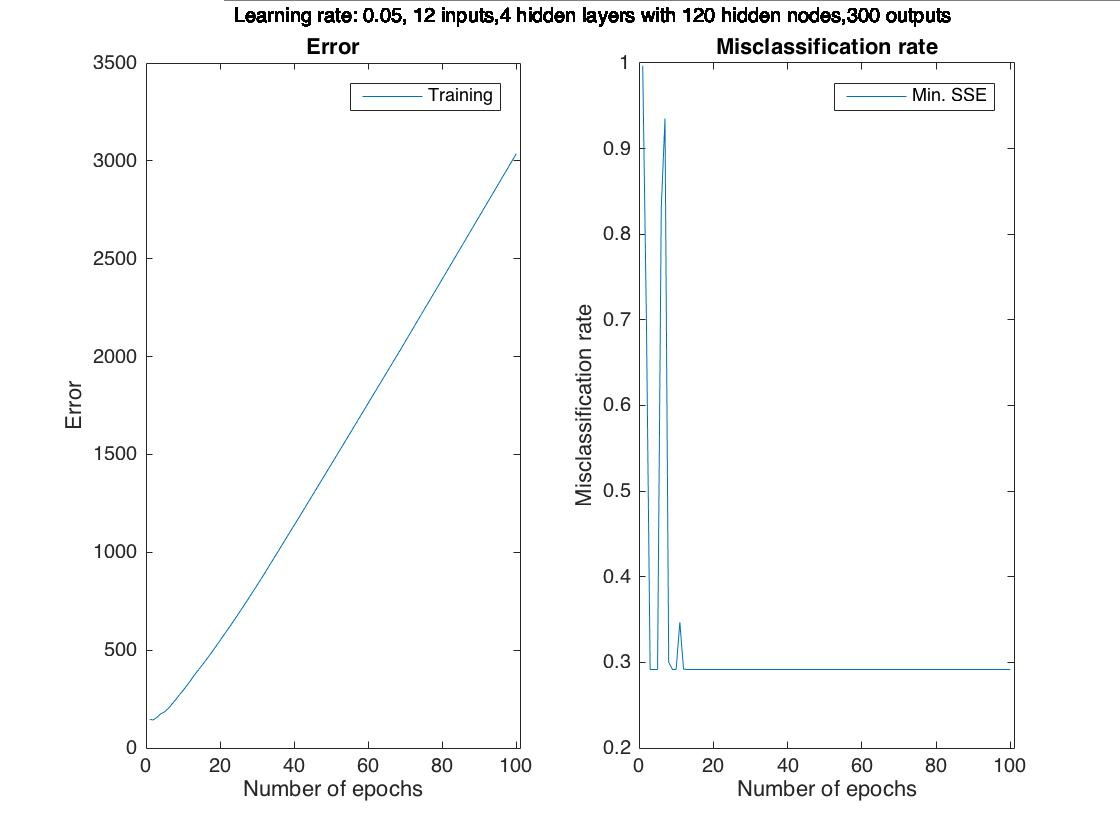
\includegraphics[scale=0.45]{images/ann/horribleResultsWIth300Outputs}

\subsection{Better Performance of Neural Network: Only 5 Output Nodes}
\label{subsec:annBetterPerformance}
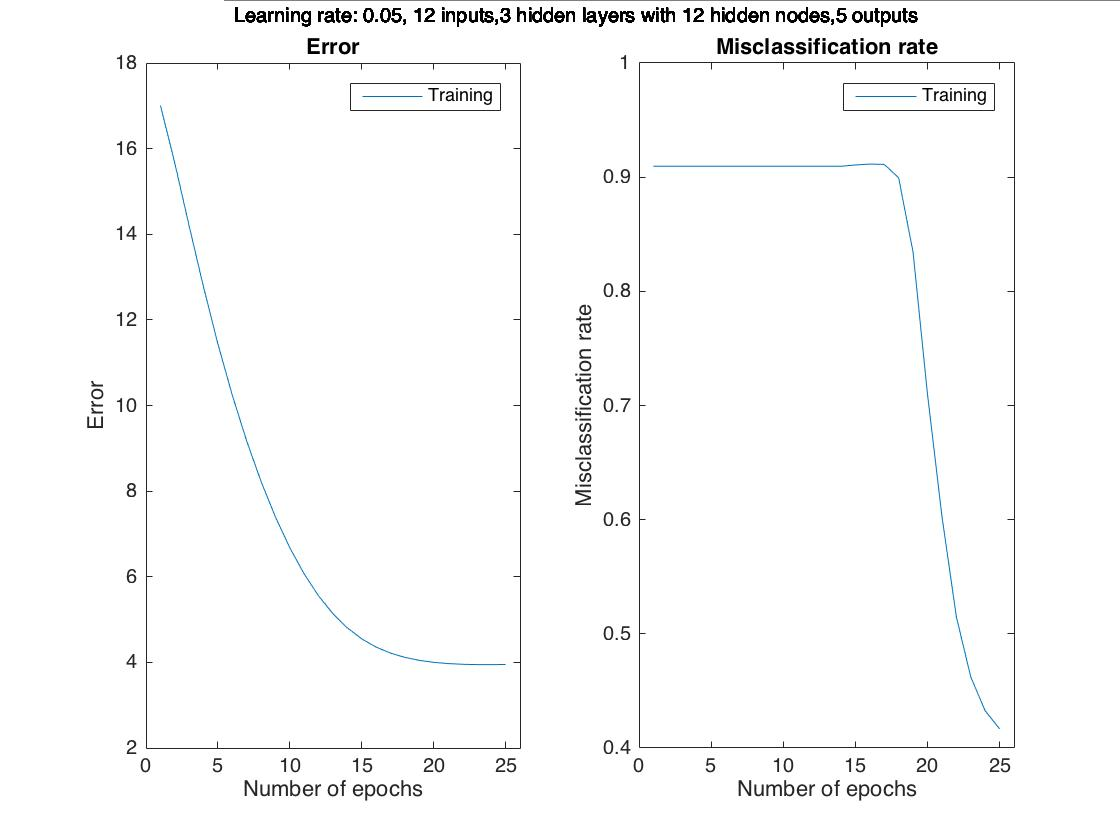
\includegraphics[scale=0.45]{images/ann/slightlyBetterWithTop5Genres1}
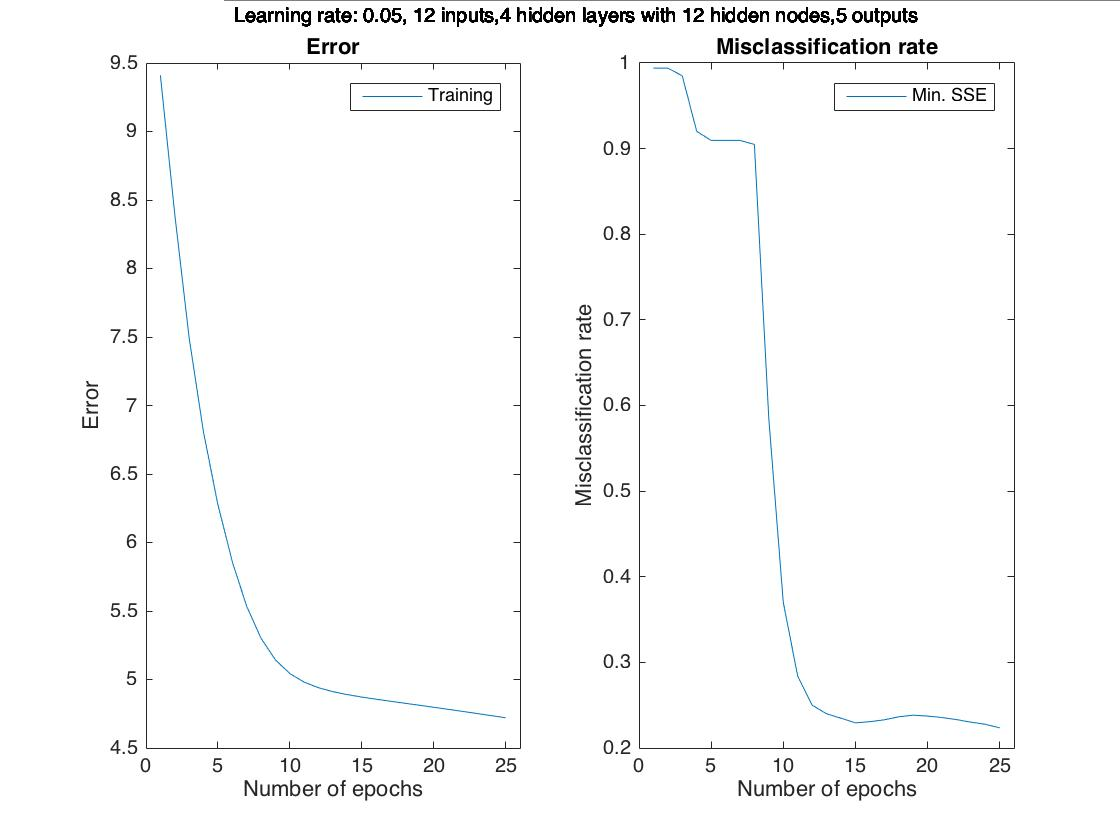
\includegraphics[scale=0.45]{images/ann/slightlyBetterWithTop5Genres2}

\subsection{Performance of Various Neural Networks: Only 1 Output Node}
\label{subsec:variousANN}
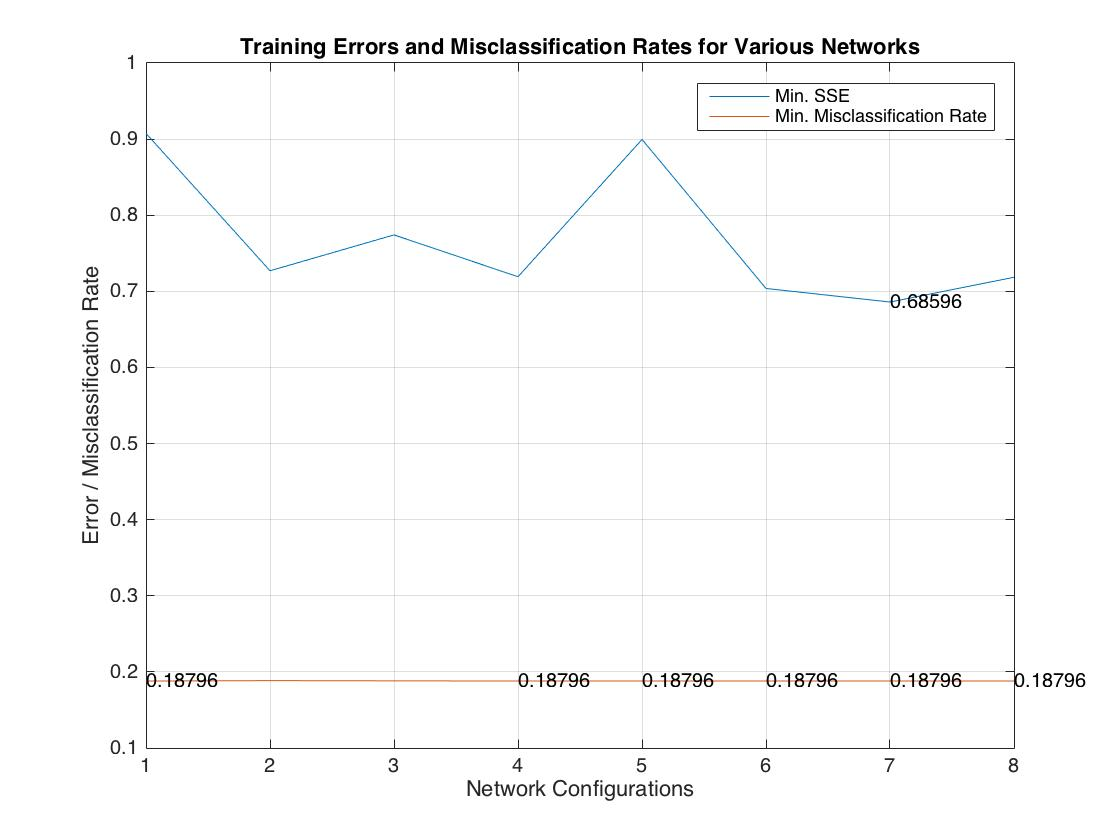
\includegraphics[scale=0.45]{images/ann/graphOfVariousNetworksWith1Genre}
Each of the networks that were tested to yield the graph above contained 12 input nodes and a single output node for the classification of rock songs. The various hidden layer and learning rate configurations are provided below. The numbers correspond to the x-axis values in the graph above. 
\begin{enumerate}
    \item 3 hidden layers, each with 9 hidden nodes, and a learning rate of 0.05
    
    \item 3 hidden layers, each with 9 hidden nodes, and a learning rate of 0.1
    
    \item 3 hidden layers, each with 12 hidden nodes, and a learning rate of 0.05
    
    \item 3 hidden layers, each with 12 hidden nodes, and a learning rate of 0.1
    
    \item 4 hidden layers, each with 9 hidden nodes, and a learning rate of 0.05
    
    \item 4 hidden layers, each with 9 hidden nodes, and a learning rate of 0.1
    
    \item 4 hidden layers, each with 12 hidden nodes, and a learning rate of 0.05
    
    \item 4 hidden layers, each with 12 hidden nodes, and a learning rate of 0.1
\end{enumerate}

\subsection{Best Performance of Neural Network: Only 1 Output Node}
\label{subsec:annBestPerformance}
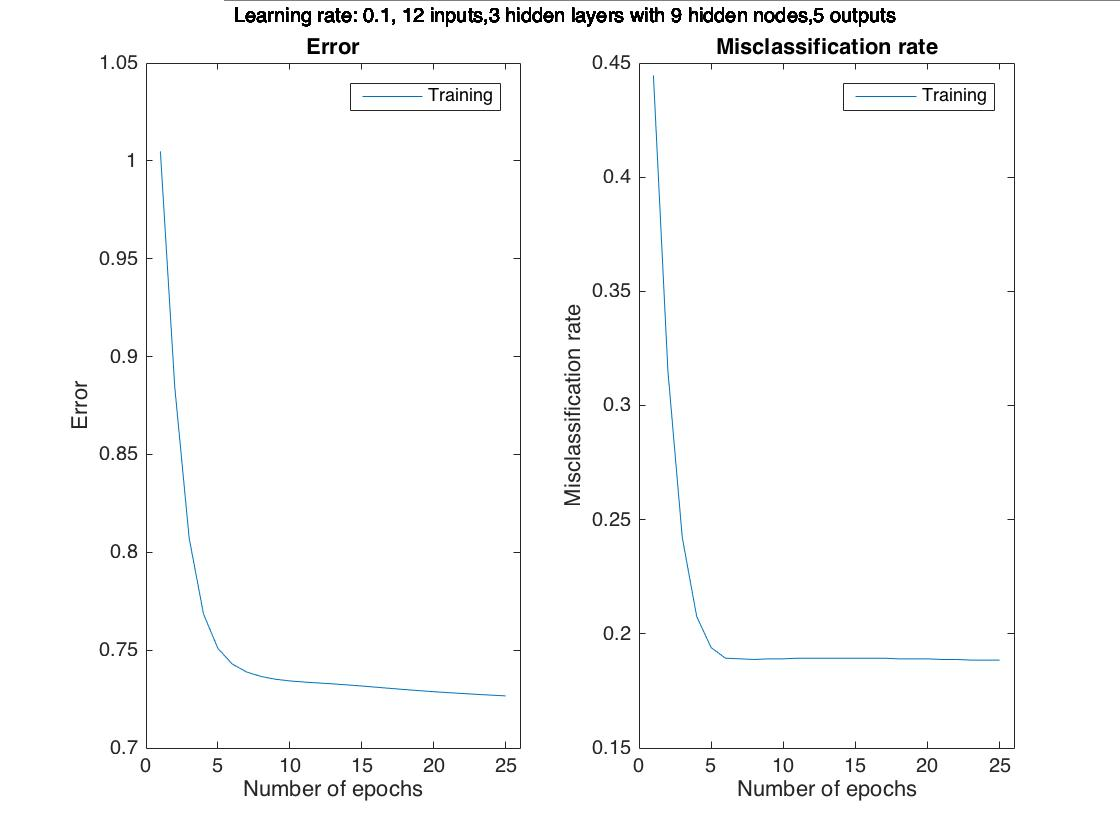
\includegraphics[scale=0.45]{images/ann/bestRun}



%%%%%%%%%%%%%%%%%%%%%%%%%%%%%%%%%%%%%%%%%%%%%%%%%%%%%%%%%%
%%%%%%%%%%%%%%%%%%%%%%%%%%%%%%%%%%%%%%%%%%%%%%%%%%%%%%%%%%
\pagebreak
\horizontalLine
\section{Code}
\label{sec:code}

\subsection{Main Loop for Testing Different Neural Network Architectures}
\label{subsec:annLoop}
\begin{lstlisting}
% Declare different values for hidden layers/nodes
% and learning rates
hiddenLayerValues = [1 2 3];
hiddenNodeValues = [30 60 90 120];
[~, inputs] = size(x);
[~, outputs] = size(y);
networks = [];
rates = [0.05 0.075 0.01 0.03 0.05 0.07 0.1];


% Iterate throughout the various hidden layer/node values
% and various learning rate values
for layerValue = hiddenLayerValues
    for nodeValue = hiddenNodeValues
        for rate = rates
        
        % Initialize the architecture of the network
        architecture = [inputs repmat(nodeValue, 1, layerValue) outputs];
        
        % Construct and train the network
        [network, L] = constructAndTrainNetwork(architecture, rate, x, y);
        end
    end
end
\end{lstlisting}

%%%%%%%%%%%%%%%%%%%%%%%%%%%%%%%%%%%%%%%%%%%%%%%%%%%%%%%%%%
%%%%%%%%%%%%%%%%%%%%%%%%%%%%%%%%%%%%%%%%%%%%%%%%%%%%%%%%%%
\pagebreak
\horizontalLine
\section{Author Contributions}
\label{sec:authorContributions}
\begin{itemize}
    \item Methods:
    \begin{itemize}
        \item Linear Regression
        \begin{itemize}
            \item Peggy Li
            \item Steven Mackey
            \item James Dryden
        \end{itemize}
        \item Artificial Neural Networks
        \begin{itemize}
            \item Nicholas Layton
            \item Michael Fiueroa
        \end{itemize}
        \item K-Means Clustering
        \begin{itemize}
            \item William Otwell
            \item Marshall Hampson
            \item Amos Too
        \end{itemize}
    \end{itemize}
\end{itemize}
\end{document}

